\documentclass[esd, manuscript]{copernicus} % uncomment to see what the 2 column final paper will look like.

\begin{document}

\section{The emulator}

We treat the output of the simulator $y$ as an uncertain function $f()$ of the simulator inputs $x$, so that $y = f(x)$. We wish to produce a predictive distribution for $y$ at any model input, conditional on the points already run, or the design $(Y, X)$. Throughout the study, we use a kriging function, similar to a Gaussian process regression emulator, as coded in the package DiceKriging \citep{roustant2012dicekriging} in the statistical programming environment R \citep{Rcore2016}, for prediction of climate simulator output at untried inputs.
The kriging model or Gaussian Process regression is specified hierarchically with a separate mean and covariance function. For prediction purposes, \emph{a priori} assume that the trend is a simple linear function of the inputs, and adjust with a Gaussian process. 

%\begin{equation}
$$
f(x) = h(x)^T \beta + Z(x)
$$
%\end{equation}

Where $h(x)^T \beta$ is the mean function, and the residual process $Z$ is a zero mean stationary Gaussian process. The covariance kernel $c$ of $Z$ 

$$
Cov(Z, Z') = \sigma^2 c(x,x')
$$
can be specified in a number of different ways: we use the default diceKriging option of a Matern $v=5/2$ function so that

$$
c(x,x') = (1 + \frac{\sqrt{5} | x - x'|}{\theta} + \frac{5 | x - x'|^2}{3 \theta^2})exp(- \frac{\sqrt{5} |x-x'|}{\theta})
$$

where $\theta$ describes the \emph{characteristic length scales} - a measure of how quickly information about the function is lost moving away from a design point, in any dimension. This and other hyperparameters are estimated via maximum likelihood estimation from the design $(Y, X)$, meaning that the approach is not fully Bayesian (such an approach would find posterior distributions for the hyperparameters rather than point estimates). We use Universal Kriging, with no `nugget' term, meaning that the uncertainty on model outputs shrinks to zero at the design points. 

Full details of the Universal kriging process used can be found in \citep{roustant2012dicekriging}, section 2.1, details of the kernel can be found in section 2.3, and examples of the trend and hyperparameter estimation  in section 3 the same publication. 

\subsection{Testing the emulator}
To ensure that the emulator is adequate for prediction, we need to ensure that it predicts well across the parameter space of the design $X$. We use leave-one-out cross validation (LOOCV), where each ensemble member is removed in turn, and the output $y$ predicted with an emulator constructed from the remaining design points. This type of validation quickly shows up any design points where the emulator fails badly, either in the mean prediction, or in the assessed uncertainty. This, and other standard model selection and validation metrics can be found in e.g. chapter 7 of \citep{hastie2009elements}.

Cross validation of the emulator for forest fraction shows up no significant problems in prediction of any of the global or regional forest fraction data, across the entire design, as can be seen in Fig. \ref{fig:frac_loo}.

\subsection{Two dimensional sensitivity analysis}
We can predict the implausibility at any point in parameter space, identifying regions of input space where the model output is inconsistent with the observations. For example, in Fig.  \ref{fig:taat}, two parameters are varied across the full ensemble range, while all other parameters are held at their default value. The green point marks the default input value, projected into the two-dimensional space. For this illustrative example, we use a ``tolerance to error'' of 0.1 (1 standard deviation), which is the assumed sum of observation and discrepancy uncertainty.

Using the Central African (CONGO for brevity) rainforest to estimate implausibility of each point in parameter space, we see that the standard inputs are located in a deep ``valley'' of low implausibility. Generally, the implausibility is very low at the standard settings. There are regions where implausibility may be equally low or lower, existing as planes within the multidimensional space. However, there appears to be no evidence that the standard set is implausible, given this data.

In contrast, using the Amazon as an observation, the shape of the plausible regions seems very different when projected into this two dimensional space. There are no longer valleys of NROY space, but a larger region that appears off to one side of the design input space. In addition, the standard values are often close to or at the boundaries of implausible space.


\bibliographystyle{copernicus}
\bibliography{famous.bib}

\begin{figure}[t]
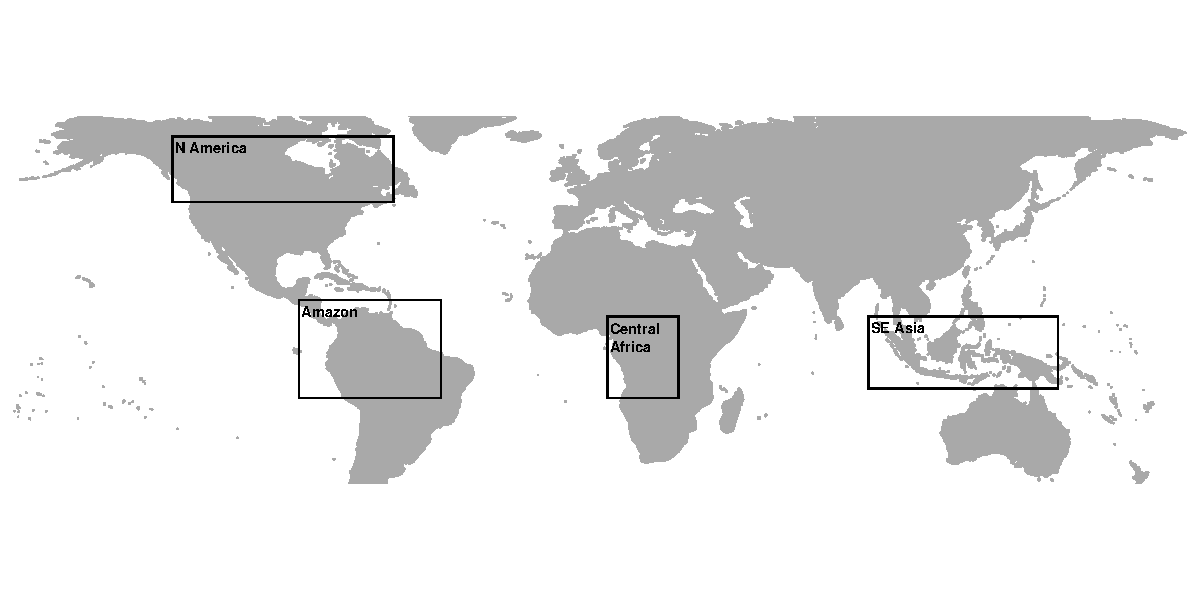
\includegraphics[width=12cm]{graphics/map_forests.pdf}
\caption{A map of the forest regions used in the study. Regions are: Amazon 15\textdegree S - 15\textdegree N, 270\textdegree E - 315\textdegree E; Central Africa; 15\textdegree S - 10\textdegree N, 7.5\textdegree E - 30\textdegree E; SE Asia 12\textdegree S - 10\textdegree N, 90\textdegree E - 150\textdegree E; North America 45\textdegree N - 65\textdegree N, 230\textdegree E - 300\textdegree E.}
\label{fig:map_forests}
\end{figure}

\begin{figure}[t]
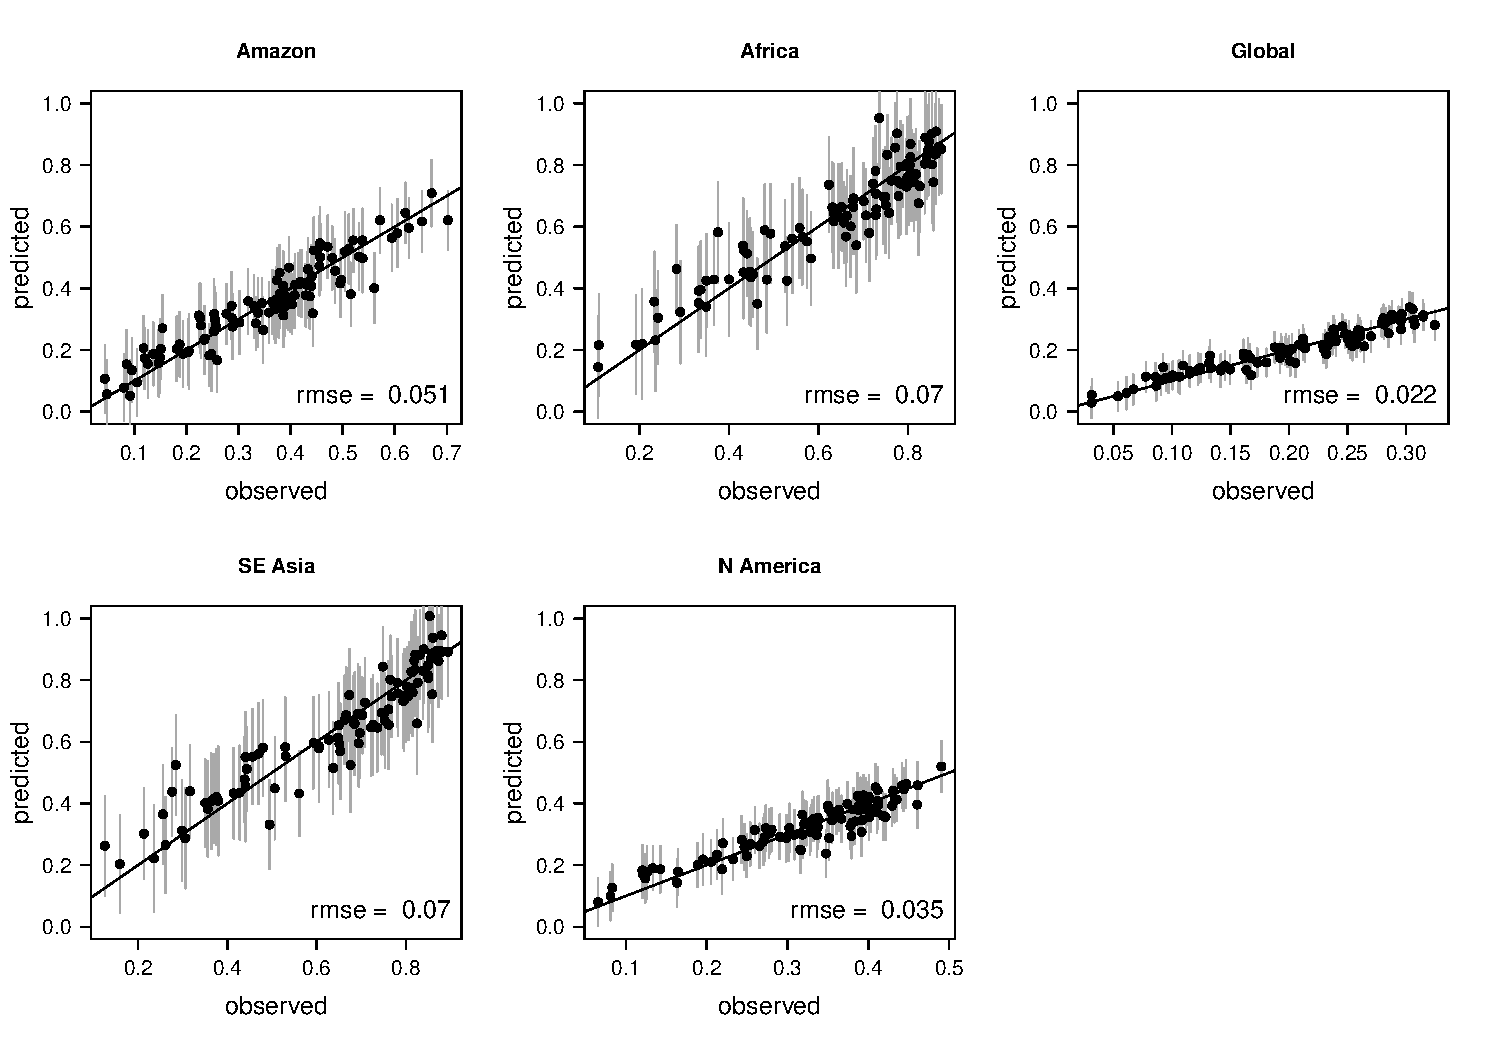
\includegraphics[width=12cm]{graphics/frac_loo.pdf}
\caption{Leave-one-out cross validation performance of the emulator, when reproducing each forest fraction. Black points represent the emulator central estimate of a held-out point, with grey lines representing $\pm$ 2 standard deviations.}
\label{fig:frac_loo}
\end{figure}

\begin{figure}[t]
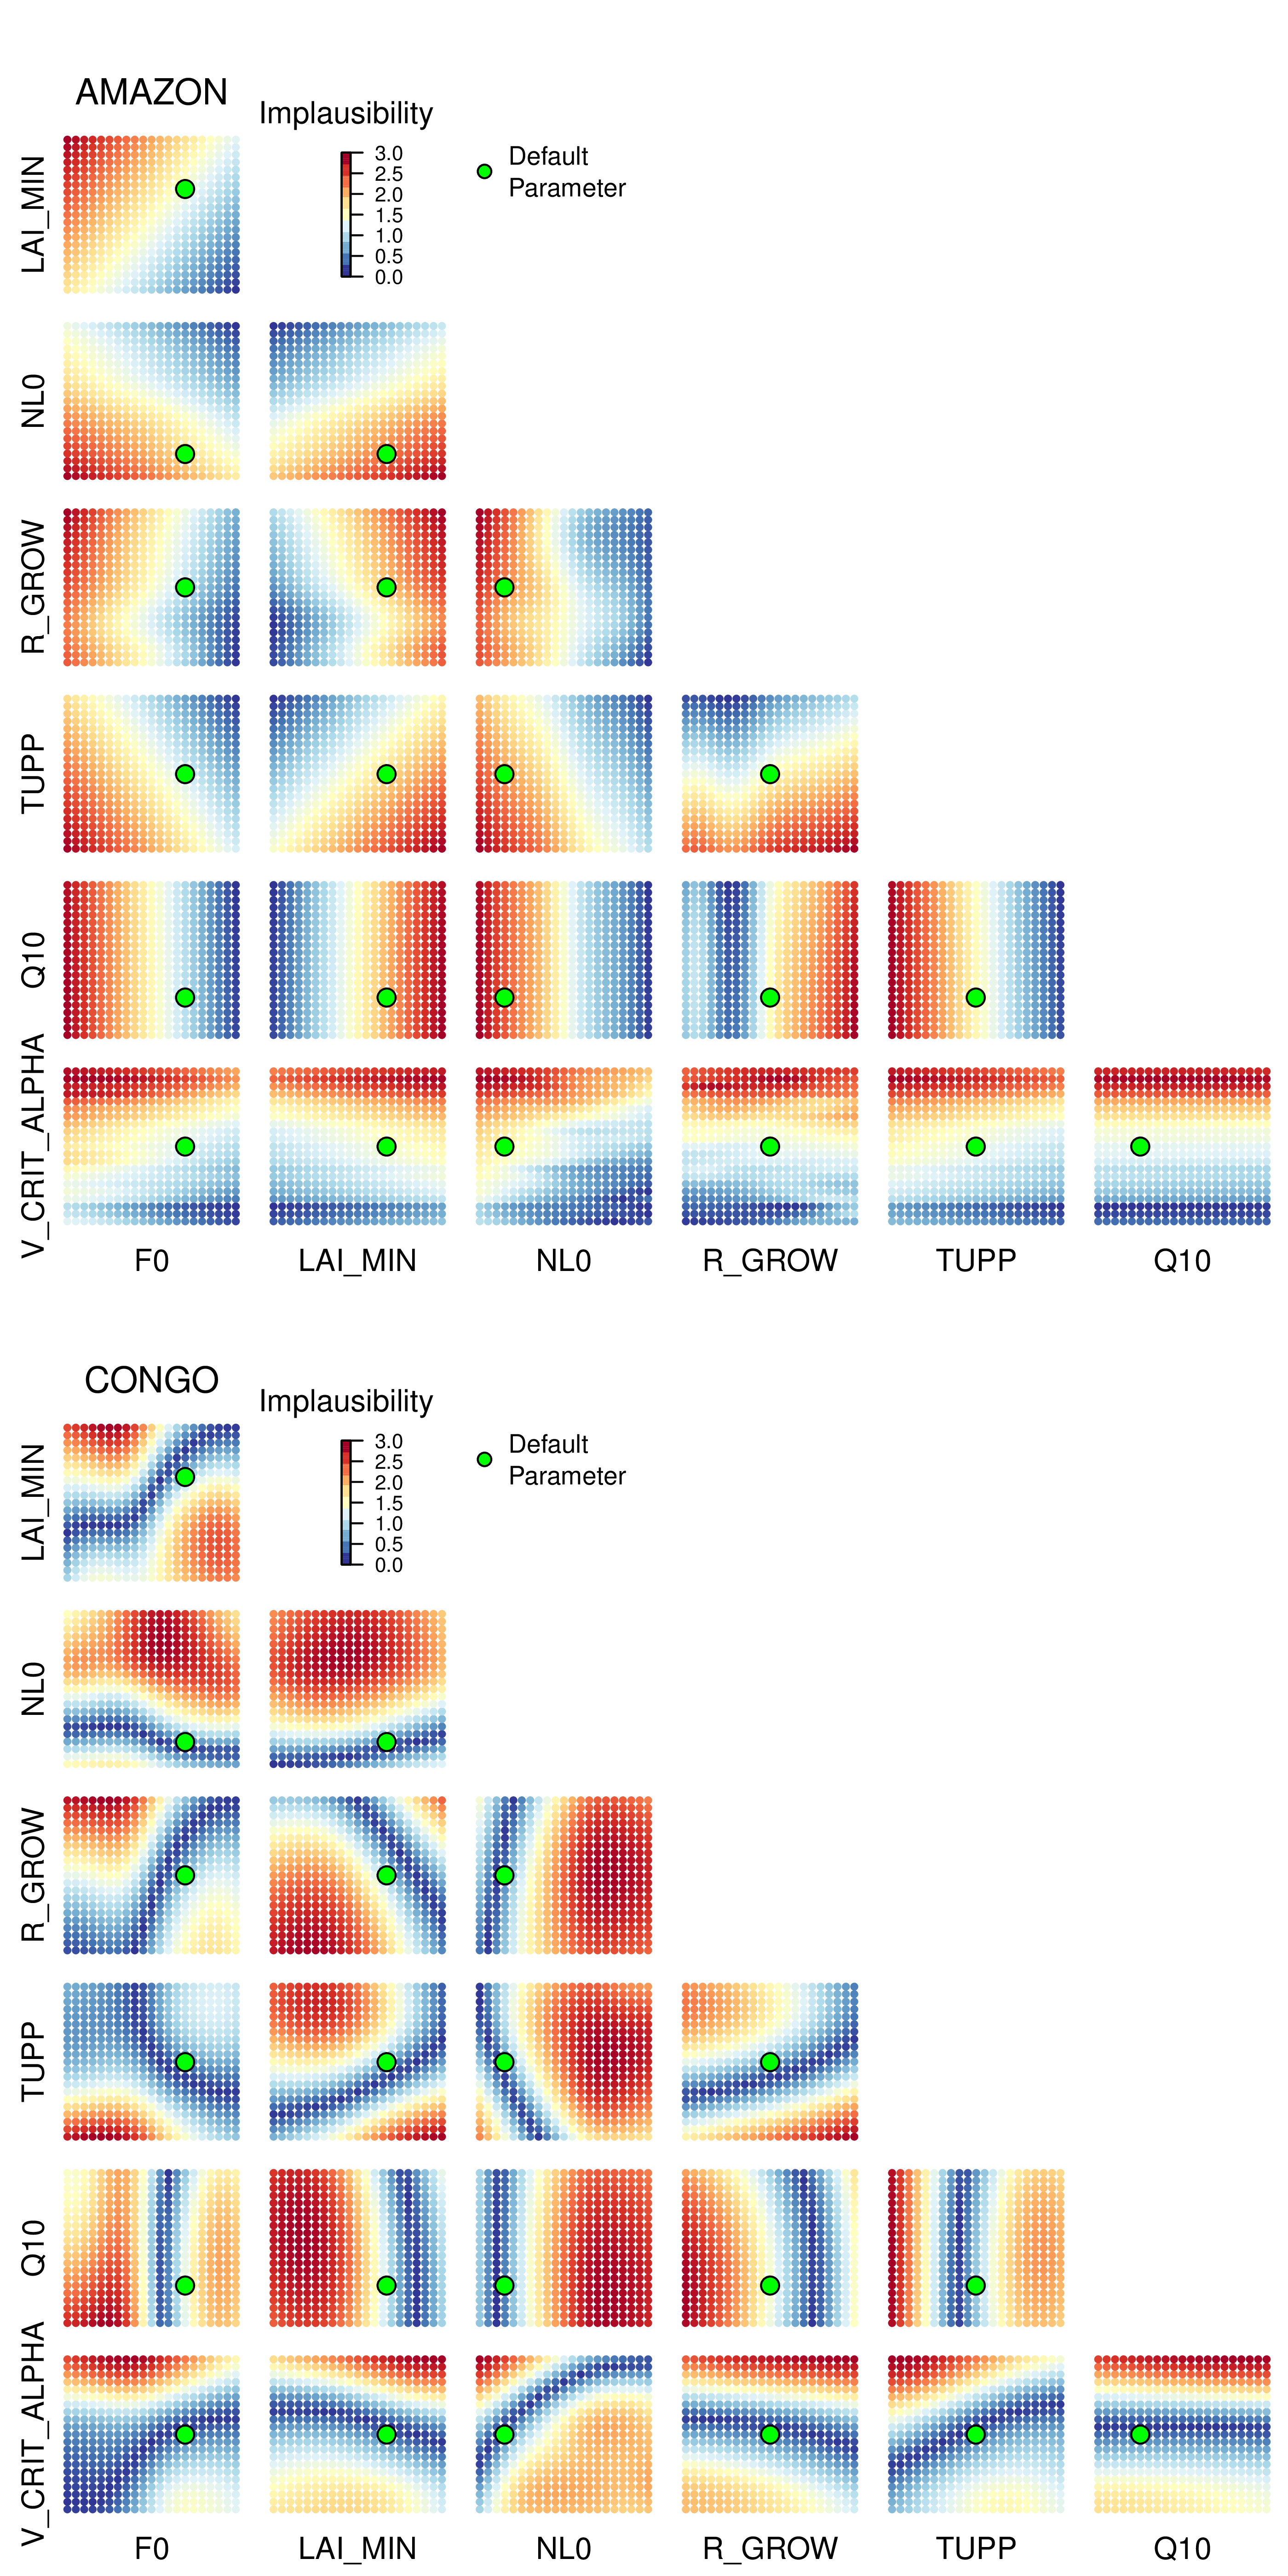
\includegraphics[width=8.3cm]{graphics/taat.png}
\caption{Implausibility, given a ``tolerance to error'' of 0.1, varying two parameters at a time and holding all others at their default values. Amazon forest (top) and Central African forest (bottom). Blue indicates regions where the model best simulates the individual option, while red indicates regions where the model simulates the forests more poorly. The green point indicates the location of the ``standard'' set of parameters for FAMOUS in the varied dimensions.}
\label{fig:taat}
\end{figure}



\end{document}